% !TEX root = main.tex
\section{Plan} % (fold)
\label{sec:plan}

This section details our plan for completing this project.
It details what parts will be done by whom, current status and the final deliverable goal.
In addition a brief timeline is included.

\begin{figure}[!ht] %[tbp]
\centering
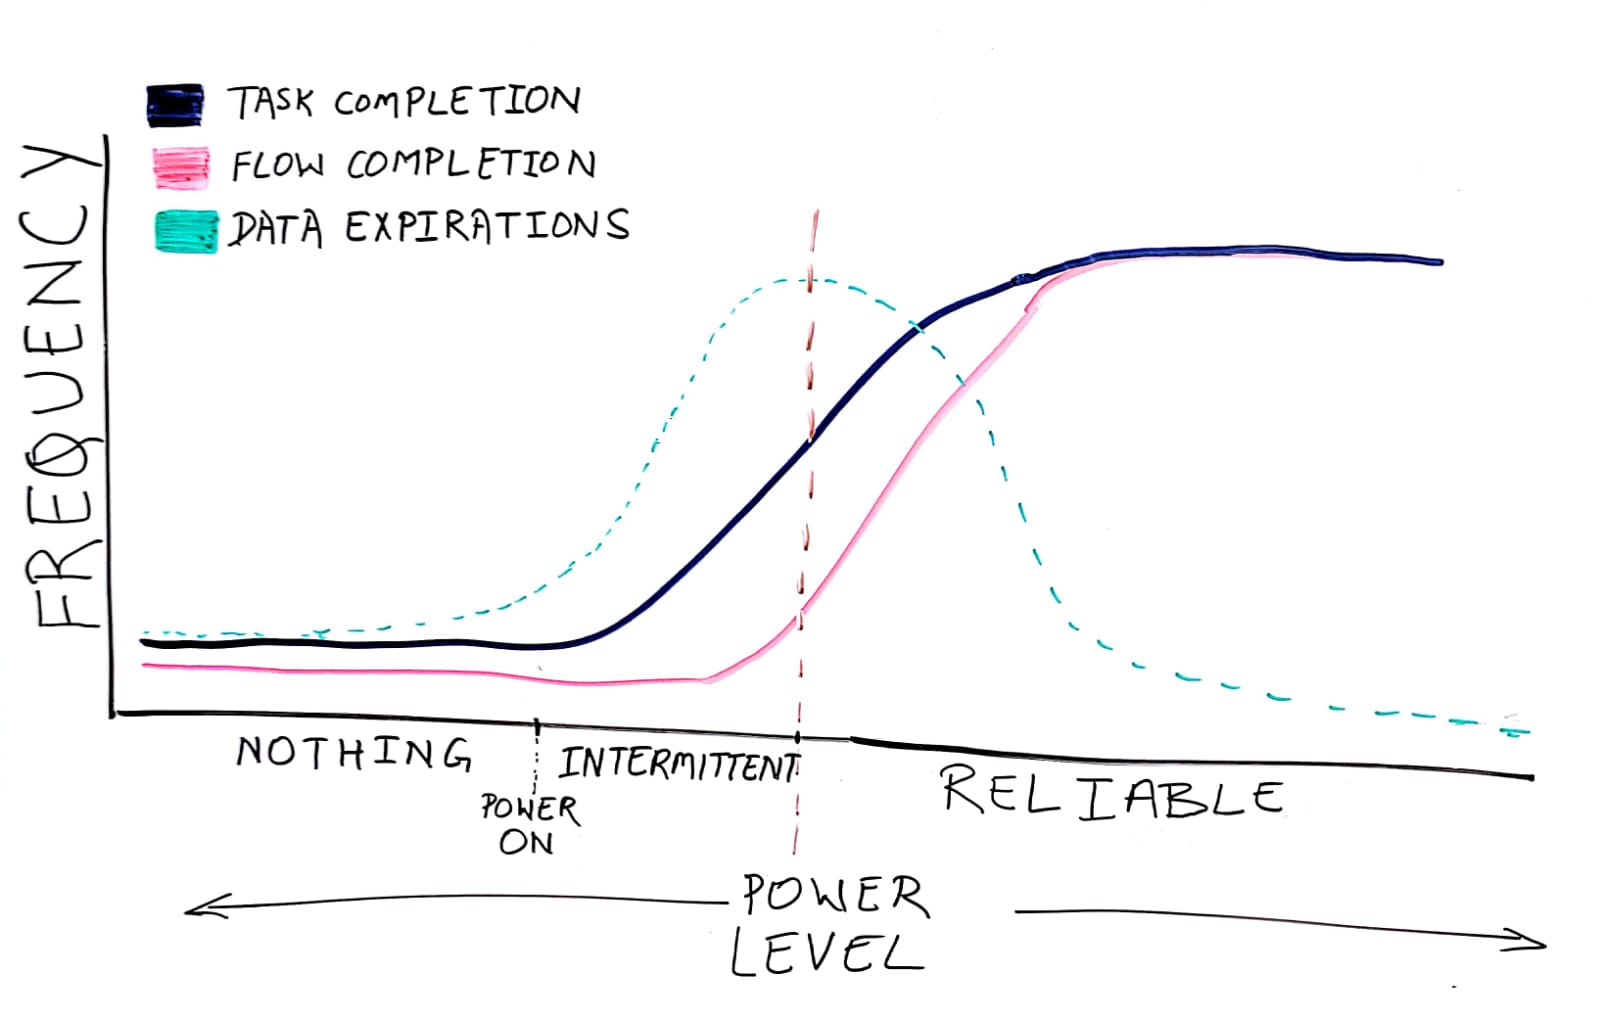
\includegraphics[width=1.0\linewidth]{Figures/graph.jpeg}
\caption{
 Data expirations, task and flow completion rate with respect to power level.
 Note the three areas of activity - none, intermittent and reliable.
}
\label{f:circuit}
\end{figure}

\begin{figure}[!ht] %[tbp]
\centering
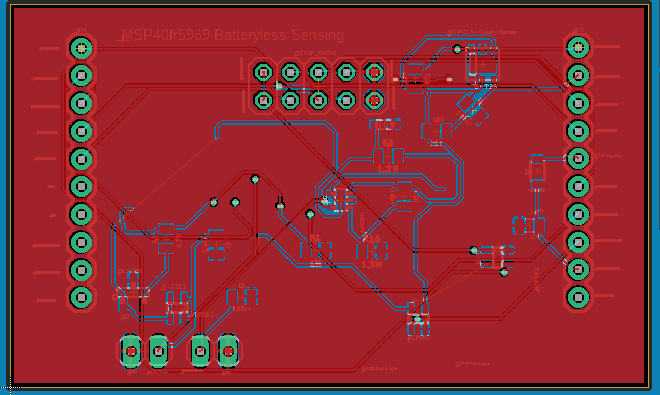
\includegraphics[width=1.0\linewidth]{Figures/circuit.jpg}
\caption{
Basic Batteryless Shield for solar powered launchpad.
}
\label{f:graph}
\end{figure}

\subsection{Work Distribution}

This section details how the work will be distributed between group members.

\subsubsection{Siddhant}
Siddhant's focus on this project is working with the usb powered MSP430.
The data received from the solar launchpad needs to be sent to a laptop computer via serial communication.
Once that channel is working he will use it to send the task and flow completion rates as well as data expirations.
This data will then be used to make the graph shown in Figure \ref{f:graph}.

\subsubsection{Lavaniyaa}
Lavaniyaa's focus on this project is working with the solar powered MSP430.
She is working on writing C code for the batteryless applications.
She will also be helping Siddhant to setup the serial communication.

\subsubsection{Ryan}
Ryan's focus on this project is working with ANTLR to build the translator that will insert the appropriate communication code for each task.
In addition, the ANTLR program must be able to identify flows

\subsection{Completed Goals}

We have designed and submitted a batteryless board for use with the MSP430 to OSHPark, see Figure \ref{f:circuit}.
We have to thank Simeon for providing us with the main file and a board to use in the interim.
The board we have submitted is a simpler version which removes UFOP, since it adds unnecessary complication to this project.
It hasn't arrived yet, but should soon.
A simple MSP430 C program have been written for simple sensor reading.
In addition, we wrote simple code to communicate the task completed to another MSP430.
Two MSP430's are connected via digital pins with the batteryless devices pins set as outputs and the battery powered devices pins set as inputs.
A simple tag grammar for task identification has been written for ANTLR.
Tags will have the following format {\tt |< Task n >|} and |</ Task n >|.
In addition, a simple java program has been written to parse inputted code.
ANTLR works using event handlers that fire when the parser reaches certain code, such as a function definition.

\subsection{In Progress Goals}

A MSP430 program for simple radio RX/TX is under progress.
Since we noticed that everyone was having difficulty with the nRF24L01+ radio we decided to use the cc1101 radio instead.
Once the boards arrive from OSHPark we will assemble them.
The ANTLR event handlers need to be implemented so that the C code can be properly injected.
We also plan to build a ruby script for ANTLR and GCC to get them to work as one compiler.
The data shall be transferred from MSP to the computer for plotting.
We shall write scripts in R to plot the charts from the data.
Once we verify that the system is working under stable power we will need to test using different solar panels.
Different lighting conditions shall be tested for the solar panels.
Specifically we will ramp up the lighting with the aim of collecting task and flow execution rates as well as data expirations for each of the three power level zones documented in Figure \ref{f:graph}.


\subsection{Risks and Unknowns}
A major risk and unknown in this project is data gathering and logging.
We haven't written code to communicate between the computer and the MSP430 receiving and storing this information may be more difficult than we anticipate.
This project is predicated on giving developers feedback so if we cannot send data to a laptop directly we will need to find an alternative method.
One potential alternative would be to save this data to an SD card instead so it can then later be read.
An additional alternative feature to add would be to use an RGB LED to indicate which power level the system is in - low power, intermittent or reliable.

\subsection{Final Semester Goals}
The final goal of this project is to have a system capable of "energy debugging" a batteryless system that uses code annotated with our task and flow language.
This debugger will be able to communicate which tasks and flows are being completed and which are not for a given IV curve.
In addition to a bigger picture graph such as the one in Figure \ref{f:graph}, the debugger will give the developer feedback on the level of completion for the program being ran currently.
